
\chapter{怪圈,或缠结的层次结构}

\section{机器能具有创造性吗?}

在第十八章,我描述过阿瑟·塞缪尔的精彩的跳棋程序,它可以击败它的设计者。据此,听一听塞缪尔自己关于“计算机与创造性”问题的感想还是很有趣的。下面引文摘自塞缪尔写于1960年的一篇反驳维纳的文章。

\begin{quote}
我坚信机器不可能具有维纳的文章所暗示的那种创造性。按照他的意思,“机器一定能够超越其设计者的某些局限性。在这种情况下,它们可能既是有效的又是危险的。”

……

机器不是精灵,它不是靠魔法工作,它不具有意愿,而且与维纳的意见相反,不会生成事先没有放进去的东西。当然,这样说不包括偶然出故障的情况。

……

机器所表现出来的“意向”是事先已明确化的人类程序员的意向,或是依照程序员所指定的规则从这些意向中导出的子意向。我们甚至可以像维纳那样期望更高的抽象层次,在那些层次上程序不仅修改子意向,而且也修改导出规则,或修改其修改规则的方式,如此等等。在那种层次上甚至一台机器会设计和构造另一台具有更强能力的机器。但重要的是,除非机器已经得到如何去做这些事的指令,否则它\emph{不会也不可能}\lnote{(黑体是他用的)}去做这些事。这里有一条逻辑上永远存在的鸿沟,一边是实现人的愿望的过程中任何一种极力的扩展和精心的构造,另一边是在机器中开发属于它自己的意愿。如果不相信这一点,则要么就相信魔法,要么就相信人的意愿只是一种错觉,而人的行为是和机器一样机械的。也许维纳的文章和我的反驳两者都是被机械地决定了的,但我拒绝这么想。\note{塞缪尔,“自动化的某些道德和技术后果——一份辩驳”,《科学》[\bn{Science}],132期(1960年9月16日出版),第741--742页。}
\end{quote}

这让我想起了卡罗尔的对话(《二部创意曲》)。我来解释一下为什么这样说。塞缪尔反对机器自我意识(或愿望)的论点是建立在这样的见解之上的:对意愿的任何机械化都需要一种无穷回归。类似地,卡罗尔的乌龟争辩说,任何一步推理,无论多么简单,如果不援引更高的层次上的规则来证实其合理性,都不能进行。但这种证实本身不是一个推理步骤,这样你不得不求助于更高层的规则,如此等等。结论:推理包含着一个无穷回归。

显然,乌龟的论证中有些不大对头的东西,而且我相信塞缪尔的论证也有类似的问题。为了显示两者的相似性,我现在暂时充当一下魔鬼的辩护士来“帮助魔鬼”,故意唱唱反调。(众所周知,上帝帮助自助者,因此想来魔鬼就只帮助那些不自助的人。魔鬼帮助他自己吗?)以下是我站在魔鬼的立场上从卡罗尔的对话中推出的结论:

\begin{quote}
“推理是不可能的”这一结论对人类不适用,因为无论有多少更高的层次,我们的确是在进行许多推理,这对任何人都是习以为常的。这表明我们人类的活动不需要规则:我们是“非形式的系统”。但从另一方面来说,上述结论可以作为一种论证,说明对推理进行机械化解释是不可能的,因为任何机械系统势必明确地依赖于规则。因此,除非有元规则告诉它何时使用规则,有元元规则告诉它何时使用元规则,如此等等,否则它不可能开始工作。我们可以断言,推理能力永远不可能机械化。它是为人类所独有的能力。
\end{quote}

魔鬼辩护士的这种观点有什么错误呢?显然是如下的假设:如果没有规则告诉机器如何去做某件事,它就做不了。事实上,机器能和人一样容易地避开乌龟那笨拙的责难,而且理由是同样的:机器和人两者都是由硬件构成的,而硬件可以按照物理学定律完全独立地运行。这里根本不需要“允许你使用规则的规则”,因为最底层的规则——关于它们不再有“元规则”——是嵌入于硬件之中的,它们的运用无需经过许可。由此可见,卡罗尔的对话说到底并没讲出人和机器的任何区别(而的确,推理是可以机械化的)。

关于卡罗尔对话就谈这些。下面回到塞缪尔的论证。其要点——如果允许我夸张一下——是这样的:

\begin{quote}
没有任何计算机真正“想要”去做任何事,因为它是被别的什么人编好了程序的。只有当它能从零开始为自己编程序——这是荒唐的——它才可能有自己的关于愿望的意识。
\end{quote}

在他的论证中,塞缪尔重蹈了乌龟的覆辙,只不过是把“推理”换成了“意愿”。他的意思是说:在任何愿望的机械化的背后,必定存在一个无穷回归——或者更糟些,存在一个封闭循环。如果这是计算机不具有自己意愿的原因,那么人是怎么回事呢?从同样的评价标准中可以推出:

\begin{quote}
除非一个人设计他自己并选择他自己的需要(同时对自己需要的选择进行选择,等等),否则他不能算是具有自己的意愿。
\end{quote}

这迫使你暂停片刻,想想你自己关于“具有意愿”这一意识是来自何方。除非你是一个唯灵论者,否则你大概会说它来自于你的大脑一块你既没有设计也没有选择的硬件。然而,你需要某些东西,而非另外一些东西,这种意识并不因此而减弱。你不是一个“自我编程的物体”(不管那是种什么东西),但你仍然具有关于愿望的意识,它发源于你的心智的物理基质之中。同样,尽管事实上不会有从“乌有之乡”自发地出现于存储器中的那种魔术般的程序(一个“自我编程的程序”),机器在某一天仍可能具有意愿。它们拥有意愿的原因和你相同——都是因为许多层次上硬件和软件的组织与结构。由此可见,塞缪尔的论证说到底并没有讲出机器和人的任何区别(而的确,意愿是可以机械化的)。

\section{每个缠结的层次结构下面都有一个不受干扰的层次}

紧接在《二部创意曲》之后,我说过本书的一个核心论题将是“言语和思维是否遵从形式规则?”。本书的主要努力之一就是要指出心/脑的多层性,并且我已试图表明对此问题的最终回答是“是的——条件是你要下到最底层——硬件——去发现这些规则。”

现在,塞缪尔的陈述引出了一个我将要继续探讨的概念。这是说:当我们人在思维时,我们的确是在改变我们自己的思想规则,同时我们改变那些修改规则的规则,如此下去——但这些都可以说是“软件规则”。最底层的规则并未改变。神经元始终以同样一种简单的方式活动。你不能“想服”你的神经元去改变活动方式,虽然你可以使你的头脑改变思想的形式和主题。正像《前奏曲,蚂蚁赋格》中的阿基里斯一样,你可以达到你的思想,但不能达到你的神经元。各个层次上的软件规则都可以改变,而硬件规则不变——事实上,软件的灵活性来自于硬件的稳固性!这里没有任何悖论,不过是一个关于智能机制的基本而又简单的事实。

在能进行自我修改的软件和不受侵犯的硬件之间的这种区别,正是我要在这最后一章中加以展开的主题。我要从中发展出一组变奏,其中有些变奏可能看起来很牵强,但我希望等到我完成这个循环,回到大脑、心智和自我意识等问题时,你会发现在所有这些变奏中都有一个不变的内核。

我在本章中的主要目的是讨论一些想象,它们帮助我形象化地设想意识是如何从错综复杂的神经元中产生。我将讨论一些难以捉摸的直觉,我希望这些直觉是有价值的,也许对别人能有所帮助,使他们能更清晰地表述他们自己关于心智活动的想象。我仅仅希望我自己思想中的关于思想和想象的模糊想象能够促成其他人思想中的关于思想和想象的更清晰的想象。

\section{一种自我修改的棋}

第一个变奏关系到这样一种棋赛:当轮到你走的时候,你可以修改规则。以国际象棋为例,显然规则始终是同样的,而每一步只是改变了局势。但让我们发明一种变形的国际象棋,在下这种棋时,一旦轮到你走,你可以走一步棋,或是对规则进行修改。可是怎么改呢?随便吗?你能把它改成跳棋吗?显然这样乱来将是毫无意义的,必须有某些限制。例如这样一种修改:允许你重新定义马的走法,让它不再走“横$1$竖$2$”(当然还有“竖$1$横$2$”),而改走“横$m$竖$n$”(或“竖$m$横$n$”),这里$m$和$n$是任意的自然数。当轮到你走棋时,你可以对$m$或$n$加$1$或减$1$。因此它可以从“$1$-$2$”到“$1$-$3$”到“$0$-$3$”到“$0$-$4$”到“$0$-$5$”到“$1$-$5$”到“$2$-$5$”……然后将会有一些规则来重新定义象的走法以及其它棋子的走法。还可以有些规则被用于在棋盘上添增新线和删除旧线……

现在我们有两层规则:一层是说明如何移动棋子的,另一层是说明如何修改规则的。这样就有了规则和元规则。下一步是很显然的:引进用于修改元规则的元元规则。但怎样才能做到这一点,这可并不显然。我们之所以能很容易地建立移动棋子的规则,是因为棋子的移动是在一个形式化空间中进行,即棋盘。如果你能为规则和元规则设计一种简单的形式化表示法,那处理它们就会象形式化地处理符号串——甚至可以像处理棋子一样。若把问题推向极端,你甚至可以用辅助棋盘上的一些位置来表示规则和元规则。那时,棋盘上的任意一种局势既可以被看成一盘棋,也可以被看成一组规则,还可以被看成是一组元规则,这取决于你用哪种方式解释它。当然,两名棋手必须在这种表示法的解释上达成协议。

这时,我们就可以有任意多个相邻的棋盘:一个用于下棋、一个表示规则、一个表示元规则、一个表示元元规则——如此上去,你愿意有多少都行。当轮到你走时,你可以在除最顶上那个棋盘之外的任何一个棋盘上走一步,这一步所遵循的规则是位于该层次结构中上一层的棋盘所提供的。无疑,两个棋手会由于几乎所有事情——虽然并非每件事情——都可以改变而被搞得晕头转向。根据定义,最顶上的棋盘是不能改变的,因为你没有规则来说明如何修改它。它是“不受干扰的”。还有一些不受干扰的东西:关于不同棋盘的解释方式的协议、轮流走棋的约定,每人每次可以改变一个棋盘的约定——如果你仔细检查这个想法,还能发现更多。

现在就有可能进一步取消使这种定位得以建立的支柱。一步一步地来……,我们首先把这一整套棋盘压缩成一个棋盘。这是什么意思呢?这就是说对于这个棋盘可以有两种解释方式:\pnum{1}作为要移动的一些棋子;\pnum{2}作为一些移动棋子的规则。轮到你走时,你移动了棋子——你必然也就修改了规则!这样,规则就会不断修改它们自己。这使我们想到了“印符遗传学”——或因此想到了真正的遗传学。在棋局、规则、元规则、元元规则之间的差别已经消失。一度整齐、清楚的层次结构变成了一个怪圈,或缠结的层次结构。棋的着法改变了规则,而规则又决定了棋的着法,鸡生蛋,蛋生鸡……虽然仍有不同的层次,但“低层”和“高层”之间的区别已经被抹掉了。

现在,有一部分过去不受干扰的东西已经成为可修改的。但仍有很多不受干扰的东西。正像以前一样,在你和你的对手之间有一些约定,据此可以把棋盘解释成一组规则。还有一个约定是关于轮流走棋的——或许还会有其它的隐含约定。因此必须注意,关于不同层次的概念以一种出人意料的方式存活下来了。有一个不受干扰的层次——在其上是关于解释的约定,还有一个缠结的层次——在其上是那个缠结的层次结构。因此这两层仍可构成一个层次结构:不受干扰层控制着缠结层上发生的事件,但缠结层没有也不可能影响不受干扰层。尽管缠结层本身是个缠结的层次结构,它仍然被存在于它之外的一组约定所控制。而这就是关键所在。

正如你无疑已经想到的那样,没有什么可以阻止我们去做那种“不可能做到”的事——那就是说,根据棋盘上的位置把关于解释的约定本身作为修改对象,以此把不受干扰层和缠结层缠结在一起。但为了进行这样一种“超缠结”,你必须和你的对手达成某些与这两个层次有关的进一步的协议——而这样做就创建了一个新层次——一个新的不受干扰的层次,它位于那个“超缠结”层之上(你愿意说“之下”也行)。这一过程可以继续进行下去。事实上,这里所做的“跳跃”很像在《生日大合唱哇乌阿乌阿……》中——或在对TNT的各种改进形式反复进行哥德尔化的过程中——所描绘的那样。每当你以为你已经达到了终点,总会有“跳出系统”这一主题的某种新的变奏出现,而想发现它则需要一种创造力。

\section{再谈作者三角形}

但我并不想进一步讨论在自我修改的国际象棋中会出现的那种极其复杂的缠结现象。我举这个例子只是想形象地说明下述观点:在任意一个系统中总存在某个“受保护的”层次,它不会被其它层上的规则所攻击,尽管这些规则之间的相互作用可能是复杂地缠结在一起的。在第四章中有个有趣的谜,它在一个略有不同的环境中表示了同样的想法。也许它会打你个冷不防:

\begin{quote}
有三个作者——Z、W和G。现在Z仅仅存在于W所写的一部小说中。相似地,W仅仅存在于G所写的小说中。更怪的是,G也仅仅存在于小说中——当然是Z写的。那么,这样一个“作者三角形”真是可能的吗?\lnote{(见\fig{134})}
\end{quote}

\begin{figure}
%\includegraphics{img_134.png}
\begin{tikzpicture}[every node/.style={draw,circle,minimum size=5mm},
  every edge/.style={draw,postaction=decorate,bend left},
  arrow decoration]
\node (W) at (0,0) {W};
\node (G) at (2,0) {G};
\node (Z) at (60:2) {Z};
\path (W) edge (Z)
      (Z) edge (G)
      (G) edge (W);
\end{tikzpicture}
\caption[一个作者三角形。]
  {一个“作者三角形”。}
\end{figure}

这当然是可能的。但这里耍了一个花招……这三个作者Z(芝某)、W(乌某)和G(吉某)全都是侯某所写的另一部小说中的角色!你可以把芝-乌-吉组成的三角形看成一个怪圈,或缠结的层次机构,但作者侯某是处于发生这个缠结的空间之外的——作者侯某某位于一个不受干扰的空间之中。虽然芝某、乌某和吉某都能直接地或间接地彼此相互作用,而且能在他们各自的小说中互相诽谤,但他们都无法接触到侯某的生活!他们甚至无法想象到他——正像如果你是一本小说中的角色,那你也无法想象该书的作者一样。如果我想描写作者侯某,我只能在书外的某个地方来表示它。这当然会带来问题,因为要描写一个东西就必须把它放进书中……不管怎么说,侯某的确是在芝某、乌某和吉某所处的世界之外的,而且应当被表示成这样。

\section{艾舍尔的《画手》}

\begin{figure}
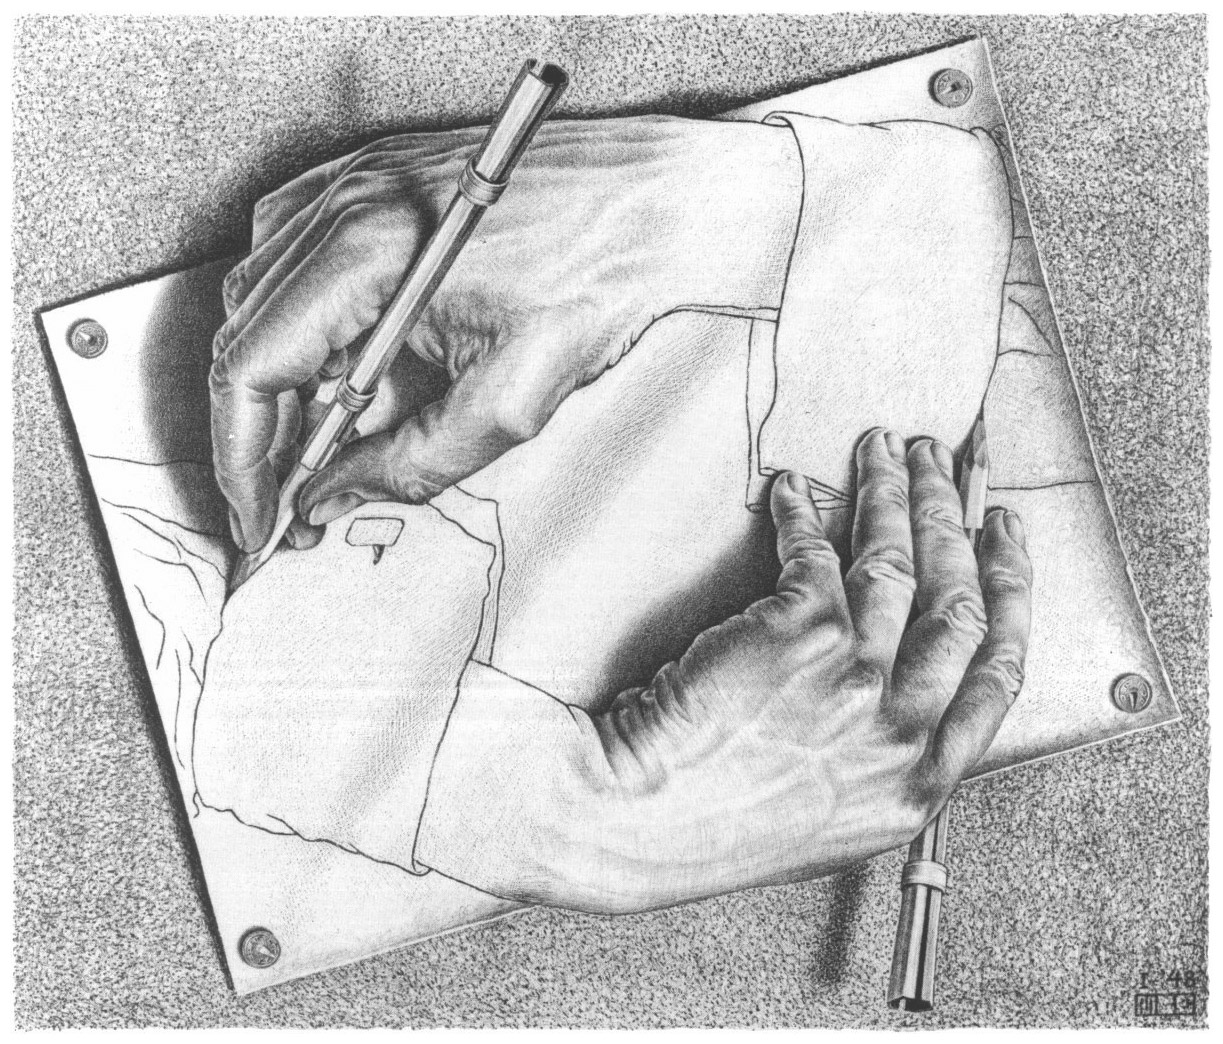
\includegraphics{img_135.jpg}
\caption[画手,艾舍尔作。]
  {画手,艾舍尔作(石版画,1948)}
\end{figure}

在我们的主题上的另一个经典性的变奏就是艾舍尔的作品《画手》(\fig{135})。在这张画中,一只左手在画一只右手,而与此同时,右手又在画左手。又一次地,平时被看作组成了层次结构的那些层次——画的和被画的——彼此重叠,构成了一个缠结的层次结构。但这恰恰说明了本章的一个主题,因为在全部这些东西之后隐藏着一直未画出但正在画的手,它属于艾舍尔,左手和右手二者的创作者。艾舍尔处于这两只手所在的空间之外,而在我为这幅画所作的示意图中(\fig{136}),你可以清楚地看到这一点。在这张为艾舍尔的画所配的示意图中,你在上部可以看到那个怪圈,或缠结的层次结构;同时,你又能在它下面看到那个不受干扰的层次,下一层使上一层成为可能。我们可以使艾舍尔这幅画进一步“艾舍尔化”,方法是拍一张一只手正在画它的照片,如此下去。

\begin{figure}
%\includegraphics{img_136.png}
\begin{tikzpicture}[every edge/.style={draw,postaction=decorate,bend left},
  arrow decoration]
\matrix[matrix of nodes,column sep=0mm,row sep=10mm,
  every node/.style={draw,ellipse,inner sep=2mm}]
{
  |(A)| 左手 & & |(B)| 右手 \\
           & \coordinate (M);\\
           & |(O)| 艾舍尔\\
};
\path (A) edge node[midway,below,font=\small]{\hbox{“画”}} (B)
      (B) edge node[midway,above,font=\small]{\hbox{“画”}} (A)
      (O) edge[dashed,bend right]
          node[very near start,left,font=\small]{画}  (A.south)
      (O) edge[dashed,bend left]
          node[very near start,right,font=\small]{画} (B.south);
\draw[decorate,decoration={coil,mirror,amplitude=.7mm,segment length=5mm}]
  ([xshift=-5mm]M-|A.west) -- ([xshift=7mm]M-|B.east) coordinate (R);
\node[align=left,anchor=south west,font=\linespread{1.1}\small]
  (UR) at ([xshift=-5mm,yshift=3mm]R) {怪圈\\或\\缠结的层次结构\\(可见的)};
\node[align=left,anchor=north west,font=\linespread{1.1}\small,below=6mm of UR] {不受干扰的层次\\(不可见的)};
\end{tikzpicture}
\caption[艾舍尔的《画手》的抽象示意图。]
  {艾舍尔的《画手》的抽象示意图,上面部分似乎是个悖论,下面部分是它的解。}
\end{figure}

\section{大脑和心智:一个神经元缠结支持一个符号缠结}

现在我们可以把这个问题和大脑以及人工智能程序联系起来了。在我们的思维过程中,符号激活其它符号,所有符号相互作用而形成异层结构的形式。更进一步来说,符号可以造成相互间的内部变化,就像程序作用于其它程序一样。由于符号组成了缠结的层次结构,这就造成了一种假象,即“不存在不受干扰的层次”。之所以有人认为不存在这样的层次,是因为它处于我们的视野之外。

如果可能画出整个这幅图像的示意图,那么其中将有一处是个庞大的符号森林,符号之间由缠结的线彼此相联,就像热带丛林中的藤蔓一样——这将是其顶层,是思维实体在其中流来流去的那个缠结的层次结构。这就是难以捉摸的“心智”层:类似于“左手”和“右手”。在这幅示意图的下端,类似于那个不可见的“原动力”艾舍尔,将会是无数神经元的表示。那个使得上面的缠结得以产生的“不受干扰的基质”。有趣的是,下面这一层本身也是个不折不扣的“缠结”——几十亿个细胞被上千亿条轴突联结在一起。

在这种有趣的情况下,一个由符号构成的软件缠结被一个由神经元构成的硬件缠结支持着。但只有符号缠结是一个缠结的层次结构。神经元缠结只是一个“简单”缠结而已。这种差别就像我在第十六章中提到的怪圈和反馈之间的差别一样。一旦一个你原以为具有规整的层次结构的系统令人惊讶地以一种扰乱了层次的方式绕了回来,一个缠结的层次结构就出现了。“惊讶”这个因素还是很重要的,正因为如此我才说怪圈是“怪”的。一个简单缠结,像反馈,并没有涉及到扰乱预先设定的层次划分。例如你在浴室里可以先用右手洗左手,再用左手洗右手,在这种情况下没有什么可奇怪的。艾舍尔并非无缘无故地选择去画画手的手!

像两只手相互洗这样的事件随时随地都在发生,我们从不特别注意它们。我对你说了几句话,然后你又回答了我几句话。这是悖论吗?不,我们的相互感知并不需要以一种层次结构作为前提,因此这里就没有什么奇怪的东西。

在另一方面,在语言谈论它自己的时候,不论这种谈论是直接的还是间接的,它的确构成了一个怪圈。在这里,某些系统之中的东西跳了出去并且作用于系统之上,仿佛它是在系统之外似的。使我们感到麻烦的大概是某种界说不清的拓扑学上的不对头:内外差别被搞乱了,就像在那个被称为“克林瓶”的著名图形中一样。尽管这个系统是一种抽象,我们的心智的确使用着带有某种精神拓扑的空间想象力。

让我们回到符号缠结上来。如果我们只看着它,忘掉那个神经元缠结,那我们似乎看到了一个自我编程序的物体——正像如果我们看着“画手”,由于忘记了艾舍尔的存在,就会产生一种错觉,好像我们看到了一幅自己画自己的图画。对这幅画而言,这种情况不太可能发生——但对于人以及他们观察自己心智的方式来说,这正是通常所发生的情况。我们“觉得”我们是在给自己编程序。的确,我们无法产生别样的感觉,因为我们被屏蔽于底层——也就是神经元缠结——之外了。我们的思维好像是在自己的空间中运行,创造新思想,而且我们从未注意到任何神经元会给我们帮助!但这是意料之中的事。我们没办法。

一种类似的双关现象可能出现在某些Lisp程序之中,这些程序被设计得可以进入并修改它们自身的结构。如果你在Lisp层上观察它们,你会说它们是在自我修改,但如果你换一个层次,把Lisp程序看成Lisp解释程序(见第五章)的数据,那么实际上只有一个解释程序在运行,而且所进行的修改只不过是对某些数据的修改。Lisp解释程序本身是不被修改的。

你应如何描述这样一个缠结的情境,这取决于你在开始描述前先要往回走多远。如果你走得足够远,那你往往可以发现能把你引向无缠结事物的线索。

\section{政府中的怪圈}

一个极有趣的有层次缠结的领域是美国政府——尤其是法院。在一般情况下,你可以想象两个辩护人就案情在法庭上展开辩论,然后由法院对案件进行裁决。法院和辩护人是处在不同层次上的。但如果法院本身卷入了一场法律纠纷,那怪事就可能开始出现了。通常存在一个处于纠纷之外的更高级的法院。即使两个低级法院卷入了某种奇怪的争斗之中,每家都声称对另一家有裁判权,这时仍有某个更高级的法院居于事外,这在某种意义下类似于我们在那种变了形的国际象棋中所讨论的不受干扰的解释协定。

但如果连最高法院自己也卷入了法律纠纷,不再有更高级的法院,这会造成什么结果呢?这和“水门事件”中发生的麻烦差不多。总统威胁说他只服从最高法院的“决定性裁决”——然后又声称他有权确定什么是“决定性的”。现在看来这一威胁并没起作用。但假如当时真的管用了,它就会在政府的两个层次之间触发一场尖锐的对抗。二者之中的每一方都可以通过某种方式合法地宣称它是“高于”另一方的——这时该找谁来确定谁是谁非呢?找国会并不解决问题,因为国会可能会命令总统服从最高法院,而总统仍有可能拒绝,并宣称他根据法律有权在特殊情况下不服从最高法院(和国会!)。这将构成一起新的法律案件,并把整个系统搞乱,因为这实在太令人惊讶、太纠缠不清——太怪了!

具有讽刺意味的是,一旦你这样碰到了房顶——也就是说无法跳出系统寻求更高层的权威,那时唯一办法是求助于那些看上去没有用规则定义清楚的力量,而它们才是更高层规则的唯一来源——这就是低层规则,在上述例子中就是指社会的普遍反应。应当记住,在像美国这样的社会里,法律制度在某种意义上是被千百万人所共同承认的一种文雅的姿态——它可以很容易地被无视,就像河水会漫过堤坝一样。那时就会出现某种程度的无政府状态。但无政府状态也有它自身的规则,而且一点也不比文明社会少:只不过它们的作用方式是自下而上的,不是自上而下的。一个研究无政府状态的人可以设法去发现某些规则,它们控制了无政府状态随时间的发展过程,而且很可能确实存在这样一些规则。

不妨用一个物理学中的现象做类比。正像本书前面提到过的那样,平衡态下的气体遵从某些简单的规律,这些规律把它们的温度、压力和体积联系起来了。但是,气体有可能违反这些规律(这就像总统有可能违反法律一样)——条件是它并非处于平衡态。在非平衡状态下,一个物理学家如果要描述所发生的情况,他只能求助于统计力学——即转到某个非宏观的描述层次。因为对气体行为的最终解释永远是在分子水平上完成的,正像对社会的政治行为的最终解释永远是在“基层水平”上完成的一样。非平衡态热力学这个领域中的研究目标就是发现一些宏观规律,以此来描述偏离平衡态的气体(以及其它系统)的行为。它和政治学中研究无政府社会所遵循的规律的那个分支相类似。

美国政府中还有另外一些稀奇古怪的缠结,诸如联邦调查局调查它本身的错误、一个县长负担着县长的责任的同时又被送入监狱、议会程序规则的自我应用,如此等等(在其它国家的政坛上也有类似的情形)。我所听说过的一个最稀奇古怪的法律案件牵连到一个自称有特异功能的人。实际上,他自称能用他的特异功能测验人的特征,这样就可以协助律师挑选陪审员。那么如果有一天这种“特异功能”被用于对他自己的审判,会出现什么情况呢?这对一个坚信“超感官知觉”存在的陪审员会产生什么影响?他会在多大程度上觉得受到了特异功能的影响(不论这种特异功能是真是假)?开拓这个领域的时机已经成熟——这里充满了自我实现的预言。

\section{与科学和鬼话有关的缠结}

谈到特异功能和超感官知觉,生活中充满了怪圈的领域就是伪科学。伪科学的所作所为总是使正统科学的许多标准信念和过程成为疑问,因此对科学的客观性构成了挑战。一些与已有的证据解释方式相竞争的新方式被提出来了,但你该怎样评价一种解释证据的方式呢?这难道不正是又回到了客观性问题,只不过是在一个更高的层次上吗?当然如此。刘易斯·卡罗尔那个无穷回归的悖论以一种新的形式出现了。乌龟可能会争辩说,如果你想说明A是个事实,你需要证据B,但你怎样确定B是A的证据呢?为了说明这一点,你需要元证据C。为了说明这个元证据的有效性,你又需要元元证据——如此令人厌烦地束缚下去。尽管有这种论点,人们还是对证据具有一种直觉。这是因为——我又要重弹老调了——人们在脑中具有预先构成的硬件,其中包括某些对证据进行解释的基本方式。我们可以在此基础上构造并积累新的证据解释方式,我们甚至要学习应该以什么方式、在什么情况下摆脱我们最基本的证据解释机制,例如我们如果想看出魔术的诀窍,就必须这样做。

关于证据的二难推理的具体例子往往和伪科学的许多现象一起出现。例如,超感官知觉常常在实验室之外得到证明,可是一旦进入实验室,它就神秘地消失了。对这种情况的标准科学解释是:超感官知觉不是一种真实现象,经不住严格的审查。但是,部分相信超感官知觉的人(绝非全部)有一种奇特的反击方式。他们说:“不,超感官知觉是真实的,只不过在人们企图对它进行科学观察时就会跑掉——它与科学世界观的本性相互排斥。”这是一种无耻的手段,我们可能该管它叫“矛头向上”,这就是说,不是怀疑手头的东西,而是去怀疑那些可靠性更高的理论。那些相信超感官知觉的人想说明:出了毛病的并不是他们的想法,而是科学的信念系统。这是一种极其狂妄的观点,除非它能找到无可置疑的证据,否则我们就要对它表示怀疑。但那样我们又遇到了同样的问题:我们在谈论“无可置疑的证据”,仿佛所有的人都能对它所指的东西保持一致意见似的!

\section{证据的本质}

在第十三章和第十五章提到过的萨哲杜-辛普利奇奥-萨尔维亚蒂缠结,为证据评价的复杂性提供了另一个例子。萨哲杜试图在辛普利奇奥和萨尔维亚蒂的相反意见之间找到某种客观的妥协,如果这是可能的话。但妥协并不总是可能的。你怎样才能“公平地”在正确和错误之间达成妥协呢?怎样才能在公平和不公平之间达成妥协?这些问题在关于日常事物的争论中一次又一次地以各种不同形式出现。

是否有可能定义什么是证据?是否有可能制订一些法律来说明应当如何从情境中生成意义?或许不能,因为任何刻板的规则无疑都会有例外,而不刻板的规则又不能算是规则。就算我们有个智能化的程序也无济于事,因为作为一个证据处理器,它会和人一样容易犯错误。因此,如果证据确实是这样一种难以捉摸的东西,那我为什么还要对解释证据的新方式提出警告呢?我是不是自相矛盾了?在这种情况下,我不这样认为。我的感觉是我们可以划出一些界线,在其外边可以进行一种有机综合。但这时不可避免地会出现某些判断和知觉——这些东西是因人而异的。它们也是“因人工智能程序而异”的。最后,还会有一些复杂的标准,它们可以被用来确定一个评价证据的方法是否得当。这包括根据这种推理方式所得到的想法的“可用性”。导致生活中的新事物的思维方式在某种意义下被认为是“有效的”。但“可用”这个词带有太强的主观色彩。

我的感觉是,我们确定事物的有效性和真实性的过程是一门艺术,它深深地依赖于一种对美和简单性的感受力,正像它依赖于坚固的逻辑或推理或任何其它能被客观地加以形式化的原则一样。我既不是说\pnum{1}真理是一种幻想,也不是说\pnum{2}人的智能本质上是无法程序化的。我是在说\pnum{1}真理是如此难以捉摸,以致于无法被任何人或人群所彻底获得,以及\pnum{2}对人工智能来说,一旦它达到了人类智能的水平——或甚至超过了这一水平——它仍将被艺术、美感及简单性等问题所折磨,而且会在它自己对知识和理解的探求过程中不断向这些目标前进。

什么是证据?这绝不仅仅是个哲学问题,因为它闯进了生活的各个领域。你每时每刻都面临着极其大量的关于如何解释证据的选择。不论你走进哪个书店或碰见个什么书摊,差不多总能看到一些关于特异功能、UFO、百慕大三角、气功治病、偏方验方、占卜、相面、黑洞、生物回授、血型测人格、心理学的新理论等方面的书。在科学界,则有关于灾变论、基本粒子理论、黑洞、数学中的真理和存在、自由意志、人工智能、简化论与整体论等等的激烈论战。在生活中实用意义更强的方面,争论的题目有维生素C的功效、石油的真实贮量(不论地下的还是库存的)、通货膨胀或失业的原因——如此等等。还有佛教禅宗、芝诺悖论、精神分析学,等等等等。从在店里把书摆在哪个架子上这种微不足道的小事,到在学校里该教给孩子们什么样的思想这种至关重要的大事,证据的解释方式都起着难以估量的作用。

\section{认识自己}

在和解释证据有关的所有问题之中,最严峻的问题之一,就是设法通过对来自外界的混乱信号的解释来说明一个人到底是谁。在这种情况下,层次内部和层次之间都蕴藏着大量的冲突。每个人的心智都不得不同时应付个人对自我评价的内在需要和外界不断流入的影响自我印象的证据。其结果是信息在人格的不同层次之间乱转,而在它转来转去的时候,其中一部分放大了,一部分缩小了,一部分否定了,一部分变形了,然后这些部分又依次被卷入到一种旋转之中,如此反复进行下去——所有这一切,都是为了要在一个人是谁和他希望自己是谁之间进行调和。(见\fig{81})

最终结局是,关于“我是谁”的完整画面是在整个精神结构中通过某种极其复杂的方式被拼出来的。而对我们每个人来说,这幅画面中都包含大量尚未解决、可能是无法解决的矛盾。这无疑提供了大量的动态张力,而这种张力对人来说起着很大作用。从这种张力之中,在关于我是谁的内部观念和外部观念之间,产生了指向各种不同目标的心理驱力,这就使我们每个人都成为独一无二的。这样一来,具有讽刺意义的是,某些为我们大家所共同具有的东西——作为具有自我反思意识的生物这一事实——反而导致了我们以各式各样的方式对关于各种事物的证据进行内在化,而这最终又成为创造不同的个性的主要力量之一。

\section{哥德尔定理和其它学科}

在人和充分复杂的形式系统间进行类比,这是很自然的,而后者和人一样,也有某种意义下的“自我印象”。\emph{哥德尔定理}说明,对具有自我印象的一致的形式系统来说,存在着某些根本性的限制。但这一定理能否具有更普遍的意义?比如说,是否有“心理学中的\emph{哥德尔定理}”?

如果我们把\emph{哥德尔定理}当做一种比喻,当做灵感的源泉,而不是企图把它逐字逐句地翻译成心理学或任何其它学科的语言,那么或许它可能会为在心理学或其它领域中发现新的真理提供启发。但把它直接翻译成其它学科中的判断,并认为后者有同样的有效性,这是不合理的。认为数理逻辑中那些极其精致的结果能不加修改地适用于一个完全不同的领域,那是个极大的错误。

\section{内省与精神失常:一个哥德尔式的问题}

我认为把\emph{哥德尔定理}翻译到其它领域之中还是有启发价值的,条件是要预先说明这种翻译是比喻性的,不能死抠字眼。在这个前提下,我发现了两种在哥德尔定理和人类思维之间建立类比的主要方式。其中之一涉及到考虑自己是否精神正常的问题。你怎样才能弄清你是否精神正常呢?这的确是个怪圈。一旦你开始探究自己精神的正常性,你就可能陷入一个极其讨厌的“信之则有”的漩涡之中,尽管这种情况绝非不可避免。每个人都知道,精神失常的人会用他们自己古怪的内部一致的逻辑去解释世界,但如果你只能用你自己的逻辑去检查它本身,那你怎样才能弄清你的逻辑是否“古怪”呢?我看这得不到任何答案。我只是由此想到了\emph{哥德尔第二定理},它说明那种断定了自身一致性的形式数论系统是不一致的……

\section{我们能否理解我们自己的心智或大脑}

我所发现的另一个关于\emph{哥德尔定理}的比喻性类比是一种有争论的见解,即认为我们最终也无法理解我们自己的心智和大脑。这种易于挑起争端的观点内容复杂,并涉及到许多层次,因此在提出它来时必须十分谨慎。“理解我们自己的心智和大脑”到底是什么意思?这可能是指要对其工作方式有个一般性的认识,就像力学对汽车的工作方式有一个一般性的认识一样;这可能是指要完全地解释为什么人们会做他们所做的一切事情;这可能是指要完全地理解人脑物理结构的所有层次;这可能是指要在一本书(或一座图书馆、一台计算机)中建立大脑的一幅完整的线路图;这可能是指要在每个时刻都精确地了解在自己大脑的神经层次所发生的事件——每次发射,每次突触传递,等等;这可能是指要写出一个能通过图灵测验的程序;这可能是指要如此完备地了解自己,以致于连潜意识和知觉这种概念都不再有意义,因为所有东西都是明摆着的;还可能是指任何别的什么。

上述自我反映中的哪一种——如果有的话——和\emph{哥德尔定理}的自我反映最为相似呢?我有点说不准。其中的某些想法很糊涂。想要做到对自己大脑状态的一切细节进行控制,这简直是白日做梦。以此为前提是十分荒唐和无聊的。如\emph{果哥德尔定理}说明上述想法是无法实现的,这也很难算是一种新发现。在另一方面,以某种深刻的方式认识自我,这个历史悠久的目标——让我们称其为“理解你自己的心智结构”——似乎还是具有一定的可能性的。但是否存在某种模糊的哥德尔式的循环,它限制着任何个人认识自己心灵时所能达到的深度?正像我们不能用自己的眼睛直接看到自己的面容一样,设想我们无法把我们完整的心智结构反映在实现它们的符号之中,这不是合情合理的吗?

所有元数学和计算理论中的限制性\emph{定理都}说明,一旦你表示自身结构的能力达到某个临界点,那就该乐极生悲了:这就保证了你永远不能完整地表示自己。\emph{哥德尔不完全性定理}、\emph{丘奇不可判定性定理}、\emph{图灵停机定理}、\emph{塔斯基真理性定理}——都具有某些古老的神话故事的味道,它们警告你说:“寻找关于自我的知识就像踏上了这样一条旅途……它并非无处不通,它不能被绘制在任何图纸上,它永无尽头,它不可描述。”

但这些限制性定理对人有意义吗?这里是对此提出异议的一种方式:我要么是一致的,要么就是不一致的(后一种情况可能性更大,但为了完备性的缘故,我两种可能性都考虑)。如果我是一致的,那又有两种情况。\pnum{1}“低保真”情况:我的自我理解低于某个特定的临界点。这已经隐含设了我是不完全的。\pnum{2}“高保真”情况:我的自我理解已达到临界点,这样就能用比喻的方式用上述限制性\emph{定理}来做类比,因此我的自我理解以一种哥德尔式的方法挖了它自己的墙角,因此我也就成了不完全的。情况\pnum{1}和\pnum{2}的前提是我具有百分之百的一致性——一种出现可能性极小的事态。更有可能的情况是我不具有一致性——但那就更坏了,因为那样在我内部就会有矛盾,而我怎么可能理解它呢?

不管一致还是不一致,任何人都无法摆脱自我的神秘性。或许我们都是不一致的。这个世界实在太复杂了,每个人都无法做到使他们的所有信念彼此协调。对一个需要快速做出许多决定的世界,张力和混乱是必不可少的。米格尔·德·乌纳穆诺曾说过,“如果一个人从未有过自相矛盾之处,那除非是他什么也不说。”我认为我们和那个禅宗大师处于相同的境地,他在一句话中出现多次自相矛盾之后,对摸不着头脑的道悟说:“吾亦不自了”。

\section{哥德尔定理和个人的不存在}

或许在我们的生活中最大的、也是最难把握的矛盾,就是下述知识:“曾经有一个时期我还不曾存在,而且还会有一个时期我将不复存在。”在某个层次上,一旦你“灵魂出窍”,把自己看成是“只不过是另一个人”,那么上述说法是完全有意义的。但在另一个层次——或许是个更深的层次——之上,个人的不存在是毫无意义的。我们所知道的一切都是嵌入在我们的心智之中的,而所有这些从宇宙中消失则是不可思议的。这在生活中是个无法回避的基本问题,也许正是\emph{哥德尔定理}的一个最好的隐喻类比。每当你企图设想你自己已不存在时,你不得不设法跳到你自己之外,即把你自己映射成另外的什么人。你想自欺欺人地相信你能够在你自己身上引进一个旁观者对你的看法,就像TNT“相信”它能把它的元理论反映在它自身之内一样。但TNT只能在一定程度上包含它自己的元理论——并非全部。而对你来说,尽管你可以幻想已经跳出你自己之外,实际上你永远无法做到——就像艾舍尔的龙无法从它所在的二维平面中跳入三维空间一样。在任何情况下,这一矛盾都是巨大的,所以我们在生活中的大多数情况下往往对它采取视而不见的态度,因为设法解决它将完全是徒劳无功的。

在另一方面,禅宗的思想揭示了这种不可调和性。他们一次又一次地面对两种信念的冲突,一种是东方式的:“我即宇宙,因此我不存在这种想法是自相矛盾的”;另一种是西方式的:“我只是宇宙的一部分,我将死去,但宇宙没有我仍会存在。”

\section{科学与二元论}

科学常常被批评为过分“西方化”或“二元化”——即渗透着主体和客体、观察者和观察对象之间的两分法。虽然科学直到二十世纪仍是仅关心那些可以完全与观察者相分离的事物——如氧和碳、光和热、恒星和行星、加速度和轨道,等等——但这个时期的科学对更现代的科学时代来说只是一个必要的序幕。在新的时代中,生命本身成了研究的对象。“西方”科学已经逐步确定不移地走向对人类精神的研究——也就是说对观察者的研究。人工智能的探索是迄今为止沿这条路线所迈出的最远一步。在人工智能出现之前,科学研究中把主体和客体相混合而产生出奇妙结果这种事有过两次主要的预演。其一就是量子力学的革命,它的认识论问题涉及到观察者与观察对象的相互干扰。另一次就是元数学中主、客体的混合,从\emph{哥德尔定理}开始,贯穿了我们讨论过的所有其它限制性定理。或许继人工智能之后的下一个步骤将是科学的自我应用:科学把自身当作研究对象。这是主、客观混合的一种不同方式——也许比人研究自己的精神更加纠缠不清。

顺便提一下,一个有趣的现象是,所有那些本质上依赖于主体和客体的聚变的结果都是限制性的结果。除这些限制性定理外,还有海森堡的测不准原理,其内容是说对一个量的测量会使得对一个相关量的同时测量成为不可能。我不知道为什么所有这些结果都是限制性的。随你怎么想吧。

\section{现代音乐与绘画中的符号与对象之别}

与主体-客体两分法密切相关的是符号-对象两分法,这已经由路德维希·维特根斯坦在二十世纪初深入地探索过了。后来“使用”和“谈论”这两个词被用来完成同样的区分。蒯恩等人也曾对记号和它们所代表的东西之间的联系进行了详尽的讨论。但对这个深奥抽象的问题贡献了许多思想的还不仅仅是哲学家。在二十世纪音乐和绘画所经历的危机中也反映出了与这个问题的深刻联系。例如,传统上音乐与绘画是把思想和情感通过一组“符号”来表现(即视觉形象、和声、节奏或别的东西),现在的一种趋势是去探索使音乐和绘画具有不表示任何东西的能力——它们只能是存在而已。这就是说它们就是纯粹的色块或声音,而在任何情况下都不再有任何作为符号的价值。

在音乐界,由于约翰·卡奇把一种禅宗式的音响方案带了进来,他产生的影响尤其大。他的许多作品都表达一种对“使用”声音——即用声音表达情感状态——的蔑视,但他喜欢“谈论”声音——即构造一些任意的声音序列,不考虑任何先前编好的编码,以使听众通过译码把它们变成消息。一个典型例子就是在第六章中描述过的那个用多台收音机构成的《大地幻景第4号》。我不准备对卡奇评头论足,但在我看来他的许多作品似乎是用来把无意义引入音乐,而且在某种程度上,是使无意义具有意义。偶然音乐是这一方向上的一种典型的探索。有许多别的当代作曲家也走上了卡奇的道路,但似乎没人具有同样多的创造性。安娜·洛克伍德有个作品叫《钢琴在燃烧》,是这样干的——把弦绷到最紧,把它们砸得尽可能地响。在莱蒙特·扬的一部作品中,为发出所需要的杂音,要推着钢琴满台跑,还要越过障碍物,就像推着一门土炮一样。

绘画在二十世纪中也经历了许多次这种巨变。开始是对于表达的屏弃,这的确是带有革命性的:这是抽象绘画的开端。在皮厄特·蒙德里安的作品中,揭示了从纯粹的表达到最抽象的模式的逐渐发展。在这个世界习惯了非表达性的艺术之后,超现实主义出现了。这是一种古怪的大转弯,有些像音乐中的新古典主义,即把最具表达性的绘画“败坏”了,并根据全新的理由来使用它:用它来产生振动、混乱和惊愕。这个流派的奠基人是安德烈·布洛东,开始于巴黎,其中较有影响的成员有达利、马格里特、德·蔡里科、唐居伊。

\section{马格里特的语义错觉画}

在所有这些画家中,马格里特最明确地意识到了这种符号-对象关系的奥秘(我认为这是使用-谈论区分的一种深入扩展)。他以此在观众中唤起了强烈的反应,尽管观众并没有把这种区分明确地用语言这样表示出来。例如,考虑一下他在静物画这个主题上进行的奇怪变奏(\fig{137}),这幅画的标题是《常识》。在画中有一个装满水果的托盘,这正是通常表现在静物画中的那种东西,它被放在一块空白画布上。符号与事实之间的冲突是尖锐的。但这还不是嘲弄的全部内容,因为整个这个东西本身当然只不过是一幅画——事实上,是一幅画着非标准对象的静物画。

\begin{figure}
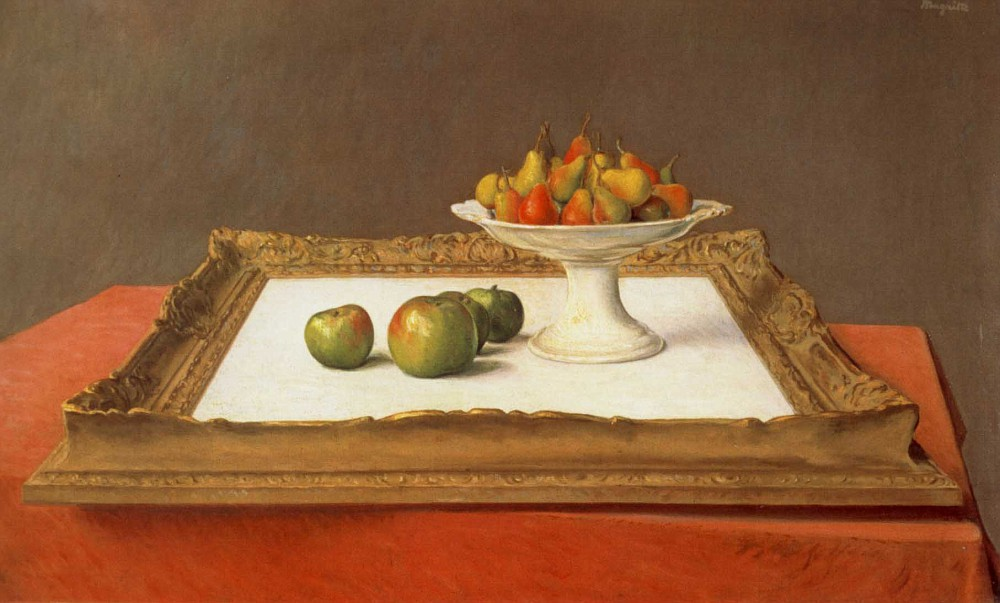
\includegraphics{img_137.jpg}
\caption[常识,马格里特作。]
  {常识,马格里特作(1945--46)。}
\end{figure}

马格里特的烟斗画系列令人既着迷又困惑。请看《两个谜》(\fig{138})。当把注意力集中在里面那张画上时,你得到的消息是“符号和烟斗是不同的”。然后你的目光转向那个浮在空中的“真”烟斗——你感到它是真的。而另一个只是个符号。但这显然全部都错了:二者都是在你眼前的同一个平面上的。如果以为一个烟斗是在一幅两重嵌套的画中,因此在某种意义上比另一个烟斗“更不真实”,那将是彻头彻尾的谬误。一旦你想“进入这间屋子”,你就已经上当了:你错把图像当成了现实。为了使你的这种轻信保持前后一致,你应当愉快地进入下一层,把图像中的图像和事实也混在一起。不受这种骗的唯一办法是把这两个烟斗都看成只不过是离你鼻子几寸远的一个平面上的一些色斑。那时,也只有那时,你才能懂得那一行字的全部含义:Ceci n'est pas une pipe[法语:“这不是烟斗”]——但具有讽刺意味的是,在所有的东西变成色斑那一瞬间,这句话也变成了色斑,因此就失去了它的意义!换句话说,在那个时刻,这幅画的语言消息以一种非常哥德尔化的方式自我销毁了。

\begin{figure}
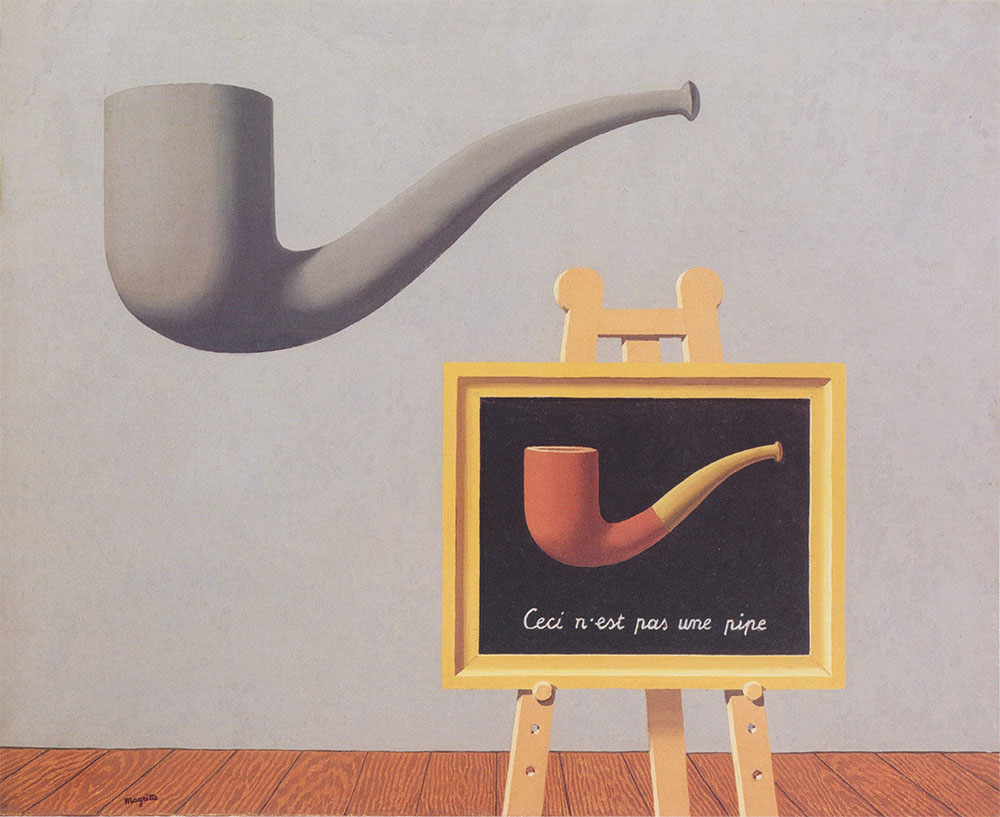
\includegraphics{img_138.jpg}
\caption[两个谜,马格里特作。]
  {两个谜,马格里特作\pnum{1966}。}
\end{figure}

《咏叹调与歌曲》(\fig{82})是取自于马格里特烟斗画系列中的一幅,它完成了《两个谜》所做的一切,不过是在一个层次上,而非两个。我所画的《以烟为号》和《如烟似梦》(\fig{139},140)构成了“马格里特主题变奏曲”。请盯着《以烟为号》看一阵,你不久就会发现一条隐藏在其中的消息:“Ceci n'est pas un message”\lnote{[法文:“这不是消息”]}。这样,如果你发现了这条消息,它就否定了自己——但如果你没发现它,你就根本没抓住要害。由于我画的这两幅烟斗都具有间接的“自我熄灭性”,它们可以不严格地对应于哥德尔串G。

\begin{figure}
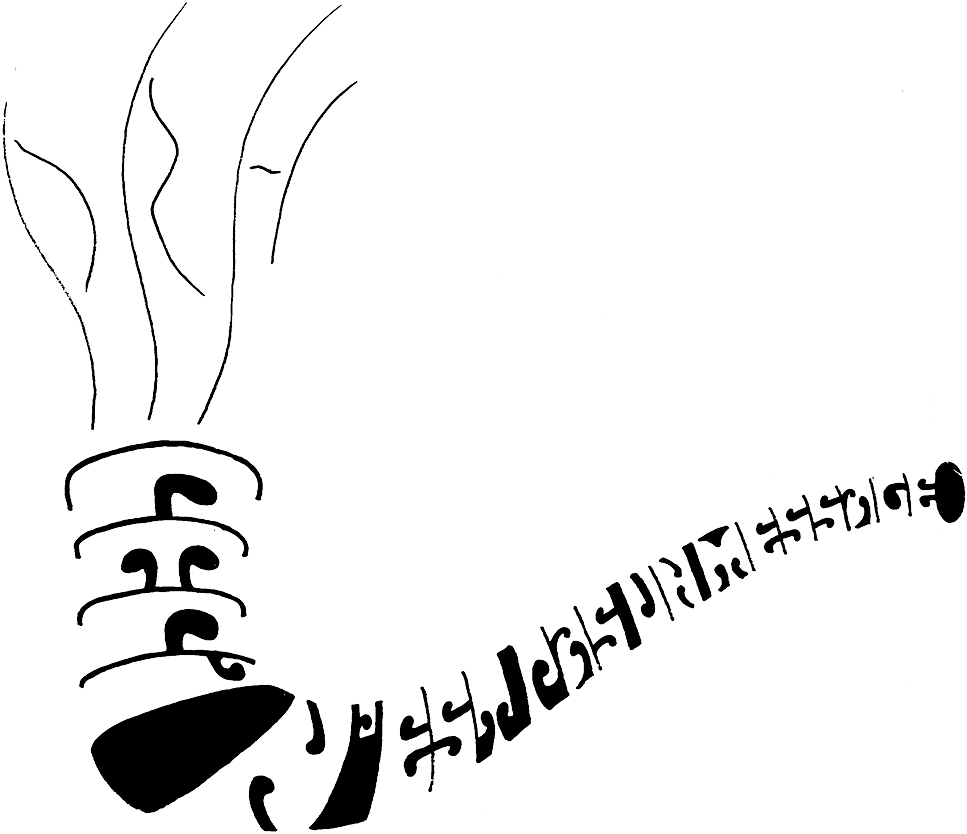
\includegraphics{img_139.png}
\caption[以烟为号。]
  {以烟为号。[作者绘] }
\end{figure}

绘画中把“使用”与“谈论”相混淆的一个经典范例就是在画中出现一块调色板。虽然这块调色板是画家的表示技巧所创造出来的错觉,但这块画出来的调色板上的颜料又的确是从画家的调色板上来的颜料。颜料代表它自己——它不是代表任何其他东西的符号。在《唐·乔万尼》中,莫扎特使用了一个与此相关的技巧:他在乐谱中明确地写出了管弦乐队调弦的声音。与此相类似,如果我想让“我”这个字代表它自己(而不是作为我的符号),我就把“我”直接写进我的文章中,然后我给“我”加上引号。这就得到一个“‘我’”(而非“我”或‘“‘我’”’)。明白了吗?

\begin{figure}
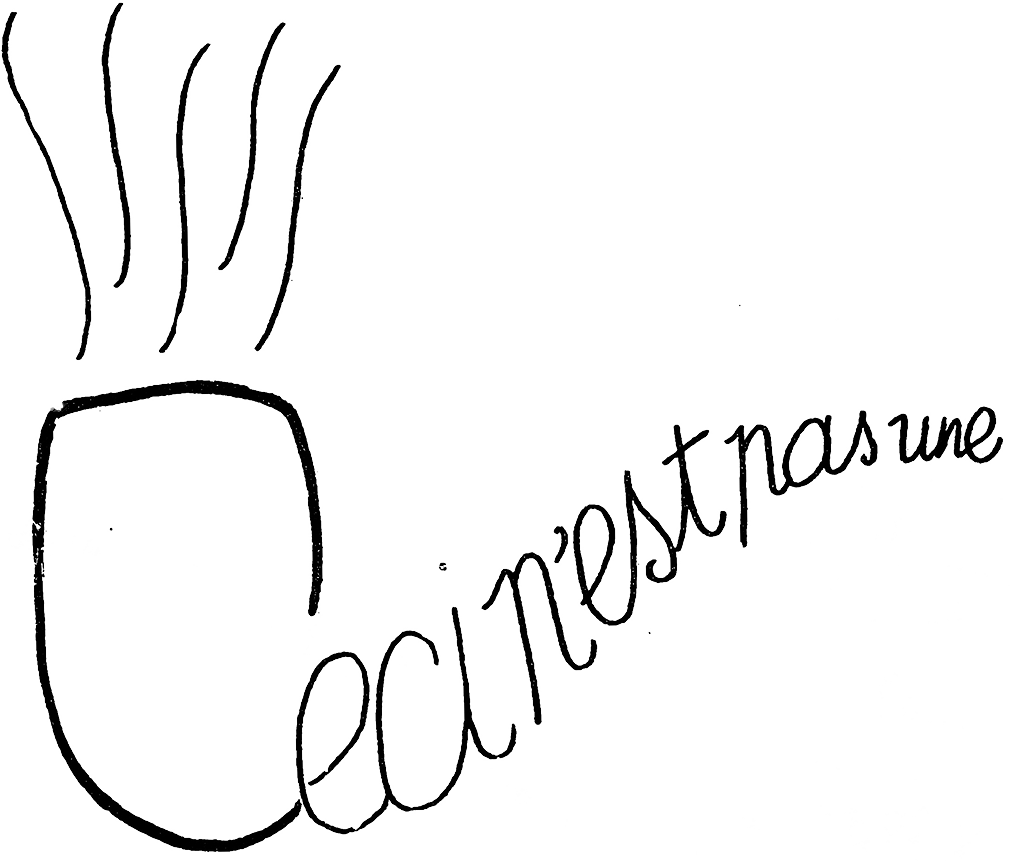
\includegraphics{img_140.png}
\caption[如烟似梦。]
  {如烟似梦。[作者绘] }
\end{figure}

\section{现代绘画的“编码”}

有许多颇有影响的人物参与了对绘画中的符号一对象二元论的进一步探索,没人能无一遗漏地把这些人的特点都列举出来。毫无疑问,对禅宗抱有浓厚兴趣的约翰·卡奇对绘画也像对音乐一样产生了重大影响。他的朋友贾斯泊·约翰斯和罗伯特·罗斯琴伯格为了探索符号和对象之间的区别,直接用对象作自己的符号——或反过来说,用符号自身作为对象。所有这些常识都可能导致下述观念的瓦解:绘画与现实之间有一段距离——或者说绘画通过“编码”来说话,而观众必须像译员那样来接收。这些现代画家的想法是取消翻译这个步骤,让对象本身呈现出来,仅此而已。如果这就是他们的目的,那他们可碰了个大钉子,而且这可能是无法避免的。

一旦一个对象在画廊中展出或被称为一件“作品”,它就会带有一种意味深长的气氛——不论你怎样告诫观众不要寻求它的意义。实际上事与愿违,你越告诉观众不要把这些对象神秘化,他们越觉得神秘。不管怎样说,如果一个放在博物馆地板上的破木箱只不过是一个放在博物馆地板上的破木箱的话,那看门的为什么不把它拖出去扔进垃圾堆呢?为什么还要标上一个艺术家的姓名?为什么这个艺术家想让艺术失去神秘性?为什么不把外面的那块烂泥也标上一个艺术家的名字?这是在捉弄人吗?是我疯了,还是这些艺术家疯了?越来越多的问题会涌入观众的脑海,他无法不这样想。这就是艺术品本身自动造成的“框架效应”。谁也没办法抑制好奇的心智产生疑虑。

当然,如果其目的是灌输一种禅宗式的观念,即认为世界既无规律也无意义,那这种艺术品大概仅仅能作为——就像用理智把握禅宗思想的效果那样——一种催化剂,其作用是激发观众灵感,使他们跳出作品之外,了解这种主张抛弃“内在意义”、把世界作为一个整体来把握的哲学。在这种情况下,从短时期看,这种艺术品是挖了自己的墙脚,因为观众的确是在考虑它的意义,但它在一些人身上达到了长期目标,即把他们引向了它的来源。但不论在哪一种情况下,说不存在把思想传送给观众的编码,这都不是真的。实际上,这是一种更复杂的编码,其中表述了诸如“没有编码”等等的东西——也就是说它部分是编码、部分是元编码,如此等等。在这些非常禅宗式的艺术对象中传送了一个消息的缠结的层次结构,或许这就是许多人以为现代艺术晦涩难懂的原因。

\section{再谈主义}

卡奇领导了一个旨在打破艺术与自然之间的界线的运动。在音乐上,主题就是认为所有音响都是平等的——一种声音民主主义。这样看来“无声”恰如“有声”同样重要。列奥纳德·毕·迈尔在他的著作《音乐、美术与思想》中,把这场运动称为音乐中的“超验主义”,他写到:

\begin{quote}
如果区分艺术和自然是种错误的举动,那么审美评价就会是毫无意义的。这样,一首钢琴奏鸣曲和一块石头、一场雷雨、一个海星相比,并没有更高的价值。卢西诺·伯里奥\lnote{[一位现代作曲家]}曾写到:“使用范畴的判断,例如对与错、美与丑这些音乐美学中的典型理性思维方式,已经不能再被用来理解一个当代作曲家在创作可听形式和音乐活动时的动机和过程。”
\end{quote}

接下来,迈尔进一步描述了超验主义的哲学立场:

\begin{quote}
……所有事物在所有时空条件下都不可避免地相互联系在一起。在宇宙中发现的任何区别、分类或组织都是随意的。世界是一个复杂、连续、单一的事件。\note{列奥纳德·迈尔,《音乐,美术与思想》,第161,167页。}\lnote{[这里能看见芝诺的影子!]}
\end{quote}

我觉得用“超验主义”作为这场运动的名字未免过于冗长。我用“主义”来代替它。由于“主义”一般是某个词的后一部分,用它作名字正好暗示了一种没有内容的意识形态——对这种意识形态不论你做怎样的揭示,都是一样的。主义是体现在艺术中的禅宗精神。正如禅宗的中心问题是要揭出自我的本来面目一样,二十世纪中艺术的中心问题似乎是要指出艺术到底是什么。上面提到的那些东冲西撞的行为正是其同一性危机的部分表现。我们已经看到,使用-谈论两分法一旦推向深入就会转化为符号-对象二元论这一哲学问题,而这又与思维之谜相联系。马格里特为他的画《人类的处境I》(\fig{141})写过下面的话:

\begin{quote}
我在一间屋子的窗前放了一幅画,从屋内向外看去,画的内容恰好表现了这幅画所遮挡住的那一部分风景。因此,画上那棵树表示着被画挡住的那棵位于屋外的树。而在观众的脑海里,它的存在既表示屋里画中的那棵树,同时又表示外面真实景色中的那棵树。我们正是这样看世界的:我们把它看作存在于我们之外,尽管它只不过是我们在内心中所体验到的一个对于世界的心智表示而已。\note{苏自·加布利克[Suzi Gablik],《马格里特》,第97页。}
\end{quote}

\begin{figure}
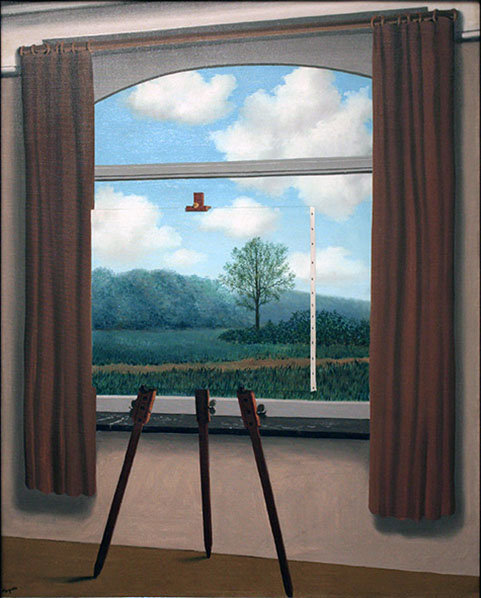
\includegraphics{img_141.jpg}
\caption[人类的处境I,马格里特作。]
  {人类的处境I,马格里特作\pnum{1933}。}
\end{figure}

\section{理解心智}

首先通过画中含蓄的图像,然后又通过直接的语言,马格里特表述了下列两个问题间的联系:一是“符号是怎样工作的?”,二是“我们的心智是怎样工作的?”因而他又把我们带回到那个前面提出的问题:“我们是否有希望理解我们的心与脑?”

我们是否会遇到某种阻止我们理解我们的心智的魔怪似的哥德尔式命题?如果你并未接受对“理解”的一种完全非理性化的定义,那我看在最终理解我们心智的旅途上就不会有哥德尔式的障碍。例如,期望着能理解大脑的一般工作原理,就像我们理解汽车发动机的一般工作原理那样,我认为是完全合理的。这完全不同于试图理解任何特定大脑的每个具体细节——更不必说试图对自己的大脑做到这一点了!我看不出\emph{哥德尔定理}怎样才能对这种设想的可行性产生影响,不管对\emph{哥德尔定理}怎样解释都是这样。我看不出\emph{哥德尔定理}能用何种理由来限制我们刻划与核实那种发生在神经细胞介质上的思维过程的一般机制的能力。我看不出\emph{哥德尔定理}怎么会设置障碍,阻止我们在计算机(或它们的后代)之上实现各种能获得和大脑大致相同结果的符号处理功能。那种试图把某个特定的人的心智复制在一个程序中的想法完全是另外一个问题——但构成一个智能程序却是一个有限得多的目标。\emph{哥德尔定理}并没有禁止我们通过程序再现我们自己的智力水平,正像它并没有禁止我们通过DNA中遗传信息的传递,再继之以教育,以再现我们自己的智力水平一样。实际上我们在第十六章中已经看到,一个非常哥德尔化的机制——蛋白质和DNA构成的怪圈——恰好是使智能得传递的条件。

这样说来,\emph{哥德尔定理}是否与我们关于自己心智的思考毫无关系呢?我想还是有关系的。尽管作用不像某些人所想象的那样神秘和具有限制性。我认为对哥德尔的证明进行理解的过程,理解那些涉及了任意编码的构造、复杂的同构、高低不同的解释层次、以及自我反映的能力,会在我们关于符号和符号处理的表象中注入某种丰富的底蕴和风味,这将深化我们对于不同层次上的心智结构之间关系的直觉。

\section{智能是碰巧不可说明的吗?}

在提出哥德尔证明的一种在哲学意义上迷惑人的“应用”之前,我想先介绍一下智能的“碰巧不可说明”性。这种观点含义如下:我们的大脑可能与汽车发动机不同,是一个我们以任何方式也无法分解的难以对付的系统。在目前这种时候,我们不知道我们的大脑是否能通过反复尝试而被劈成整齐的层次,其中每一层都能用更低的层次加以解释——或者我们的大脑是否可能挫败我们的所有进行分解的尝试。

但即使我们在自我理解时遭到失败,在其背后也并非一定有某种哥德尔式的“缠绕”。这可能仅仅是命运的一种偶然结果,是由于我们的大脑碰巧未能强到能理解它自身。不妨以鸡为例,它们的大脑虽然是远远低于自我理解所要求的水平,但仍和我们自己的脑很相像。事实上,螃蟹、树獭、食蚁兽的大脑——甚至乌龟或某种远比我们聪明的未知生物的大脑——可能都基本上在用同一组原理进行操作。螃蟹所具有的智能可能远远低于理解那些原理是怎样相互结合以产生出心智的特性所需要达到的某个阈值,而人可能离那个阈值更近一些——或许正好在它下面,甚至可能在它上面。关键之处是,并没有根本性的(即哥德尔式的)理由说明那些特性是不可理解的,它们对更高级的智能生物来说可能是一目了然的。

\section{不可判定性与高层观点不可分离}

除去这种关于脑的碰巧不可说明性的悲观看法之外,哥德尔的证明能为我们解释我们的心与脑提供哪些见解呢?哥德尔的证明提供了这样的观点:一个系统的高层观点可能会包含某种在低层上完全不具有的解释能力。我这样说是这个意思:假设某人给你哥德尔的不可判定串G,形式上是TNT中的一个串。再假设你对哥德尔配数法一无所知。你所要解答的问题是:“为什么这个串不是TNT的一个定理?”。现在你对这种问题已经很熟悉了,例如,如果对于$S0=0$问你同一个问题,你可能有一种现成的解释:“它的否定$~S0=0$是一个定理”。这样,再加上你知道TNT是一致的,就解释了为什么所给出的串是个非定理。这就是我所谓的“TNT层次上的”解释。请注意,这完全不同于对"WU"为什么不是"WJU"系统的一个定理的解释:前者是在"J"态,后者是在"W"态。

现在G怎么样呢?能处理$S0=0$的TNT层上的解释对G无能为力,因为$~\moG$不是一个定理。那些对于TNT没有整体观点的人搞不懂他为什么不能依照规则生成G,因为作为一个算术命题,它看上去没有任何毛病。事实上,一旦G变成了一个被全称量词约束的串,对G中的变量用数字去替换所得到的每个例都可以被推导出来。解释G的非定理性的唯一途径是发现哥德尔配数概念,在一个完全不同的层次上来看TNT。想在TNT层次上写出解释决不单是困难和复杂的问题,而是根本不可能做到。这种解释根本就不存在。在TNT层上从根本上看缺乏一种为更高层次所具有的解释能力。可以说,G的非定理性本质上是一个高层事实。我猜测所有不可判定命题都是这种情况,这也就是说:每个不可判定命题实际上都是一个哥德尔语句,它通过某种编码在某一系统中陈述了它自身的非定理性。

\section{意识是一种高层所具有的现象}

这样看来,哥德尔的证明就提示了——虽然绝非证明了!——可能存在某种观察心与脑的高层方式,涉及到在低层不出现的概念,而且在这个层次上可能会有在低层次上不存在——甚至从原则上讲也如此——的解释能力。这将意味着某些事实在高层可以很容易地得到解释,但在低层则根本不行。无论一个低层陈述被搞得多长、多复杂,它也无法对问题中涉及到的现象加以解释。这可以类比于下面这个事实:如果你在TNT中反复推导,不论你搞得多长、多复杂,你也绝不可能推出G来——尽管事实上在一个更高的层次上你能看到G是真的。

这种高层概念是什么东西呢?许多具有整体论或“唯灵论”倾向的科学家和人本主义者早就提出,“意识”就是一种无法用大脑成分来加以解释的现象,所以至少它可以算一个候选者。另一个更令人迷惑不解的概念是“自由意志”。因此这些性质大概是“浮现”出来的,也就是说,对它们的解释不能仅借助于生理学来完成。但关键是要明白,如果我们在提出这种大胆的假说时想要得到哥德尔证明的引导,我们就必须把这一类比贯彻到底。尤其至关紧要的是,要记住G的非定理性是有一个解释的——它不是一个彻头彻尾的谜!这个解释依赖于同时在不止一个层次上进行理解,同时一个层次上的理解方式要反映它的元层次,还依赖于这种反映的结果。如果我们的类比是成立的,那么“浮现”的现象就会变得可以根据心智系统的不同层次的关系来进行说明了。

\section{意识的核心是怪圈}

我确信,对我们大脑中那些“浮现”出来的现象——例如想法、希望、表象、类比、以至于意识和自由意志——的解释都基于一种怪圈,一种层次相互作用,其中顶层下到底层并对之产生影响,而与此同时它自身又被底层所确定。换句话说,是不同层次之间的一种自我强化的“共鸣”——正像汉肯句子那样,只是通过断定自己的可证明性,使它真的变成可证明的了。自我成为一种存在的时刻也恰是它具有反映自身能力的时刻。

上面的观点不应当被看作是一种反简化论立场。它只是意味着,一种对心智的简化论解释,如果要成为可理解的,就必须引进像层次、映射、意义等等“软”概念。原则上,我不怀疑存在着关于大脑的彻底简化论的、但却是极其费解的解释,问题在于怎样才能将其翻译成为我们自己所了解的语言。当然我们不要一个根据粒子的位置和动量所作出的描述,我们想要一个把神经活动与“信号”(中层现象)联系起来的描述——然后再把信号联系于“符号”和“子系统”,包括那个预先假设其存在的“代表自我的符号”。这种从低层物理硬件到高层心理软件的翻译类似于从数论判断到元数学判断的翻译。你还会记得,正是在这个翻译中出现的层次构成了哥德尔的不完全性和汉肯句子自我证明的特征。我猜测正是一种类似的层次交叉造成了我们几乎不可分析的自我意识。

为了应付内容丰富的脑-心系统,我们必须能在层次之间随心所欲地滑移。更进一步来说,我们还必须承认各种类型的“因果关系”,即一个描述层次上的事件能以各种方式“导致”其它层次上的事件的发生。有时候说事件A“导致”了事件B,只不过是因为其中一个是另一个在别的描述层次上的翻译而已。有时候“因果关系”具有它通常所具有的意义:物理因果关系。这两种因果关系——可能还有其它种——都必须在对心智的任何解释中被承认,因为我们在精神的缠结层次结构中必须同时承认因果链的向上和向下传播,就像在中心法则映射中那样。

在我们自我理解过程的核心,将会是对我们心智中的层次结构的理解。我的立场很接近于神经科学家罗杰·斯珀里在他的《心智、大脑与人道主义的价值观》这篇精彩的文章中所表达的观点。下面是引自那篇文章中的一段话:

\begin{quote}
在我自己所设想的大脑模型中,意识被表示成一种非常真实的动因。我认为它在脑中事件的因果序列和控制链中发挥着重要作用。它在这些过程中表现为一种活跃的、起作用的力量……简而言之,它导向这样一个问题:在充斥着脑海的各种动力之间到底是谁在推着谁转。换言之,这就是要列出脑中控制成分之间的等级关系。在人脑中存在着一个由形形色色的动力所组成的世界,而且动力里面又包含着动力。在我们所认识的宇宙里,没有比这几十厘米见方的空间中所包含的东西更为复杂的现象了。……长话短说,如果我们不断沿脑中命令链向上攀登,我们会在其顶端发现那些全面组织起来的动力和大规模的脑兴奋模式,它们和心理状态或精神活动相互关联……在大脑里的这个命令系统中离顶点不远的地方……我们发现了思想。人之所以优越于黑猩猩,就是因为人有思想和观念。在这里提出的大脑模型中,一个想法或观念的潜在动力,变得像一个分子、一个细胞、或一个神经脉冲所具有的动力那样真实。思想引出了思想,并且为新思想的形成提供了帮助。它们彼此相互作用,和同一个大脑或邻近的大脑中的心理力量相互作用,而且借助于全球通讯系统,还能和千里之外的其它国家中的大脑里的心理力量相互作用。它们还和外部环境相互作用,在进化过程中产生了突破性进展,这一进展远远超过了迄今为止在进化过程中发生的其它进展,包括有生命的细胞的突然出现在内。\note{罗杰·斯珀里,《心智、大脑与人道主义的价值观》,第78--83页。}
\end{quote}

在主观语言和客观语言这两种论述语言之间有一个著名的分裂。例如,“主观的”红色感受和“客观的”红光波长。对很多人来说,这二者似乎永远是不可调和的。我不这样认为。正像关于艾舍尔的《画手》的两种观念并非不可调和一样——一种是“在系统内看”,此时两只手在互相画;另一种是从外面看,此时它们都是艾舍尔画的。对红色的主观感受来自大脑的自我感知中心,而客观的波长则属于你退出系统之外时的观察事物方式。尽管我们之中没人能退得足够远,以至于可以把一切都看成一副“大画”,但我们不应忘记这幅大画是存在的。我们应当记住,物理定律是所发生的一切的原因——它们藏在神经网络的犄角旮旯的深处,是我们高层次的内省式探究所无法企及的。

\section{自我符号与自由意志}

在第十二章中我曾提出,我们所谓的自由意志实际上是代表自我的符号(或子系统)与脑中的其它符号相互作用的结果。如果我们把符号看成上面附有意义的高层实体,那我们就可以试着解释一下符号、自我符号和自由意志的相互关系了。

为了要认识自由意志问题,一种办法是先用一个我认为是等价的问题来替换它,而这个问题相对来说涉及的概念不那么复杂,也不太引起异议。我们不再问“系统X是否有自由意志?”,而是问“系统X是否在进行选择?”。通过仔细探讨当我们把一个系统——机械的或生物的——描述成“能够进行选择”时,到底是什么意思,我想我们能对自由意志有进一步的理解。下面我们来看几个不同的系统,在各种各样的环境中,我们会觉得应当把它们都描绘成是“在进行选择”。考察这样的系统会对我们有所帮助,而且从这些例子中,我们将对“在进行选择”到底是什么意思有所了解。

让我们以下述系统作为范例:一个小球滚下一个高低不平的山坡;用一个袖珍计算器依次求2的平方根的小数展开式中的各位数字;一个能下一手好棋的复杂程序;一个机器人在走T型迷津(这种迷津中只有一处岔路,在岔路的一端放有奖品);还有一个正在对付复杂矛盾的人。

首先,小球滚下山坡时是一种什么情况呢?它是在选择吗?我想我们大家都会同意说它没有,尽管我们当中没人能预测它所走的路径,甚至连预测其中一小段都做不到。我们觉得它在实际所通过的路径之外不可能走别的路,而它只不过是被无情的自然规律所迫才这样做的。当然,根据我们组块化了的“心智物理学”,我们能够为这个小球想象出许多各不相同的“可能的”路径,而我们看到它在现实世界中只通过其中的一条。因此,在我们心智的某个层次上,我们可能不禁会觉得这个小球是在那一大堆想象的路径里“选择”了唯一的一条。但是,在我们心智中的另一个层次上,我们会本能地理解到这种心智物理学只是在我们为世界建立内心模型时起辅助作用,而使真实的物理事件序列得以发生的机制并不要求自然界在某个假想的宇宙(“上帝之脑”)中先经过一个类似的过程来制造出各种可能性,然后再在它们之中进行选择。因此我们不会把这一过程称之为“选择”——尽管我们承认在类似情况下使用这个词常常是具有实用意义的,因为它具有一些启发性。

对那个用来求2的平方根的可编程序计算器和那个弈棋程序,我们又能作何评论呢?在这里我们可以说碰到了一个“想象的”小球,滚下一个“想象的”山坡。事实上,在这种情况下反对“作出选择说”的证据要比小球那种情况更强。原因是如果你要想重复那个小球实验,你无疑会看到一条完全不同的通向山坡下面的路径;而如果你重新运行那个求2的平方根的程序,你每次都会得到同样的结果。那个小球似乎是每次都“选择”了一条不同的路径,不管你怎样精确地试图重现它初次往下滚时的条件,而那个程序每次都通过完全相同的路径。

对那个假想的弈棋程序的情况来说,存在着各种不同的可能性。如果你和某些特定的程序对弈,然后第二盘采用和第一盘完全相同的走法,这些程序也将准确地重复以前的走法,丝毫看不出学到了什么东西或具有什么变化的愿望。另外,有一些程序带有随机装置,能够产生一些变化,但并非出自于任何深切的期望。这种程序中的内部随机数发生器可以被重置成初始状态,然后就能导致同样的对局。还有一些程序的确能从它们的失误中吸取教训,而且能根据对局的结果改变它们的策略。这种程序就不会连续重复同一盘对局。当然,你也可以使时光倒流,抹去存储器中表示学习的所有变化,就像你能重置随机数发生器一样,但这样做似乎有些不太友好。此外,我们有理由怀疑,如果所有细节——当然包括你的脑——都被重置成它们初次发生时的状态,那么你就能改变你自己过去所做的决定吗?

不过还是让我们转回到原来的问题,即在这里“选择”这个概念是否适用。如果程序只不过是“滚下想象的山坡的想象的小球”,那它们是否在作选择呢?当然答案必然是主观的,不过我要说在这里所考虑的情况和小球的情况基本相同。但是,我必须补充说明,使用“选择”这个词的要求变得非常强烈,尽管你只是把这个词作为一种方便的或带启发性的简称而已。一个弈棋程序能够超前搜索许多可能的岔路,这完全不同于一个滚动的小球。这个事实使得它更像一个生物,而不像一个计算2的平方根的程序。但是,在这里仍没有深刻的自我认识——也不存在自由意志。

现在让我们接着来设想一个拥有一堆符号的机器人。这个机器人被放在一个T型迷津中。但是,给它编的程序不是让它去寻找奖品,而是让它在2的平方根中的下一位数字是偶数时就向左转弯,是奇数时就向右转弯。现在这个机器人能够用它的符号来为外部环境建立模型,这样它就能观察到它自己所作的选择。每当走到T型路口时,如果你问这个机器人说:“你知道你这次会往那边转弯吗?”它会回答说“不知道”。然后为了继续前进,它将激活它的“决策器”子程序,该子程序能算出2的平方根中的下一位数字,并据此作出决策。但机器人对决策器的内部机制一无所知——它用机器人的符号来表示时只不过是个黑箱,以某种神秘的、而且好像是随机的方式输出“左”和“右”。除非这个机器人的符号可以摸出这个决策器的“脉搏”,否则它也会对它自己所作的“选择”大惑不解的。那么这个机器人是否在作选择呢?你可以设身处地的去想想。如果你被封装在一个滚下山坡的小球里,完全无法影响它的滚动路径,但能够用你全部的人类智能去观察它,你是否会觉得这个小球通过的路径与某些选择有关呢?当然不会。除非你的思想在影响着结果,否则即使有符号存在也无济于事。

因此,现在我们要对我们的机器人做一个修改:我们允许它的符号——包括自我符号——被用来影响所作的决定。那样,在这个完全依照物理定律运行的程序的例子中,就似乎比前面那些例子更多地深入了选择的本质。当这个机器人自己的组块化“自我”概念出现后,我们就开始与这个机器相认同了,因为它的所作所为与我们相似。它不像计算2的平方根时那样,似乎不用任何符号来控制作出决定的过程。诚然,如果我们在一个相当低的层次上来看这个机器人的程序,那和平方根程序也差不多。它也是一步一步地执行,最后输出“左”或“右”。但在一个较高的层次上我们可以看到,事实上符号正在被用来摹写环境和影响决定。这就极大地影响了我们对这个程序的看法。在这个阶段,“意义”已经进入了视野——正像我们用我们自己的心智所处理的那种意义一样。

\section{一个层次交错的哥德尔漩涡}

这时,如果外边的某个动因建议这个机器人下一次选择“左”,这个建议就会被送到那一大堆彼此纠缠不休的符号中去。在那里,它将被无情地吞没在与自我符号的相互作用之中,就像一叶小舟被吸进漩涡一样。这就是系统中的漩涡,那里,所有层次都相互交错。这时,那个“左”碰到了一个符号的缠结层次结构,并在层次间被上下传送。自我符号并不能控制它的所有内部过程,因此当一个实际决定出现时——“左”、“右”或系统之外的什么东西——系统将无法说清它来自何处。这不像一个标准的弈棋程序,在那种情况下程序不控制它自己,因此也就不知道它的棋步是哪里来的。在这里,程序是在进行自我控制,也具有关于它的想法的想法——但它不能控制它自己行动的每个细节,因此会对它的工作过程有一种“直觉”,但没有完全的理解。自由意志的感觉就产生于这种“有自知之明”和“无自知之明”的平衡中。

例如,让我们考虑一个作家,他想把他心理表象中的一些想法表达出来。他拿不准这些表象在他心目中是如何相互联系的,因此就不断地尝试,在表达事物时开始用这种方式,后来又用那种方式,最后才选定某种说法。但他知道这一切都是哪里来的吗?只有一些模糊的感觉。其来源像一座冰山一样,大部分都深藏在水下,是看不见的——而他知道这一点。我们还可以考虑一个作曲程序——就像我们前面所讨论过的那种——并想想什么时候我们才能觉得应当称它为一个作曲家,而不仅是一个人类作曲家的工具。或许促使我们这样做的条件是在程序内部存在着用符号表示的关于自我的知识,而且该程序在有自知之明和无自知之明之间平衡得恰到好处。这与系统是否以确定的方式运行毫无关系,使得我们将它说成是“在做选择”的是:我们是否能认同于程序运行时所产生的过程的一个高层描述。在一个低级层次上(机器语言层),这个程序看起来很像任何其它程序,而在一个高级层次上(组块化层),会浮现出“意愿”、“直觉”、“创造性”和“意识”等性质。

关键的思想是这个漩涡本身就决定了心理过程的缠结性和“哥德尔式的”特性。有人曾对我说:“关于自指等等这些东西很有趣,但你真的认为这里面有严肃的问题吗?”我当然是这样认为的。我认为最终将会发现这些问题处于人工智能的核心之中,而且是所有理解人类心智工作方式的尝试的焦点。因此,我才把哥德尔这块稀世瑰璧深深地镶嵌在我这本书之中。

\section{一个层次交错的艾舍尔漩涡}

\begin{figure}
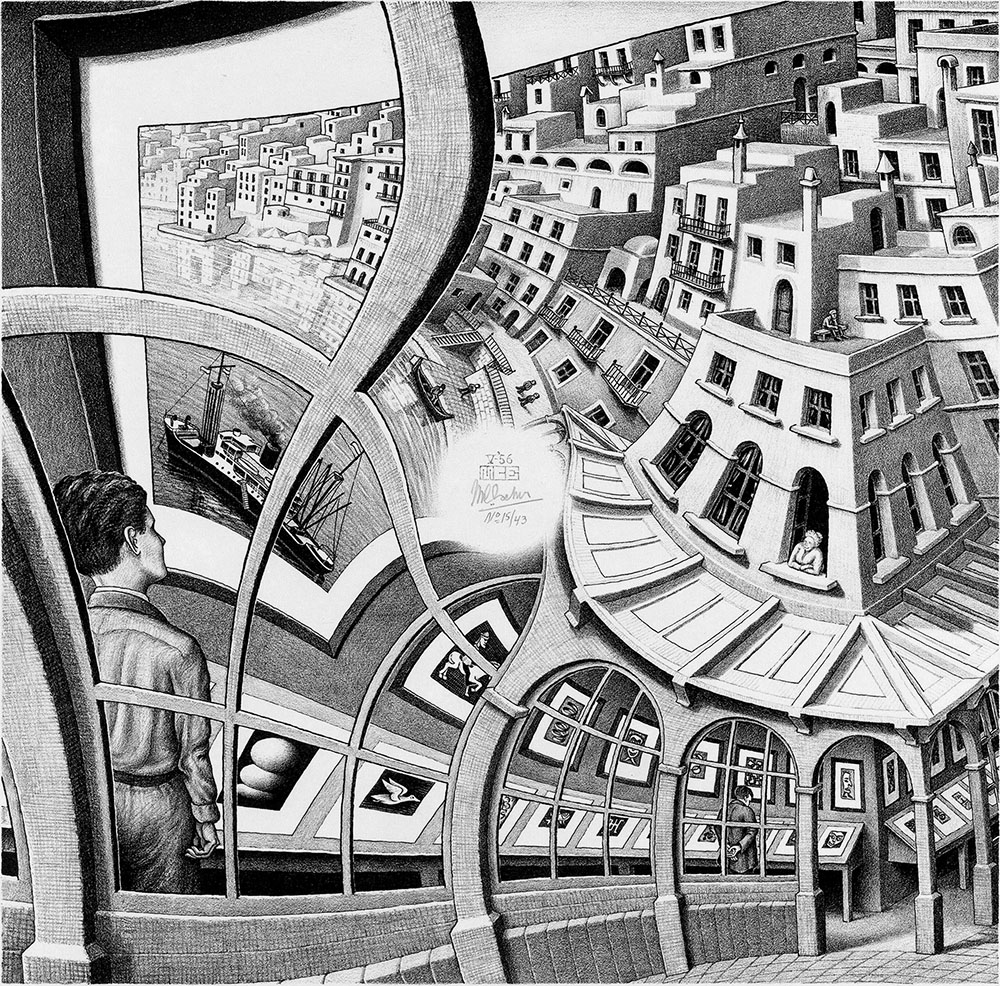
\includegraphics{img_142.jpg}
\caption[画廊,艾舍尔作。]
  {画廊,艾舍尔作(石版画,1956)。}
\end{figure}

在艾舍尔的《画廊》(\fig{142})中,为我们提供了对一个缠结的层次结构中的“台风眼”的一个美妙得令人吃惊的、同时又荒诞得令人烦乱的描绘。我们在其中所看到的是一个画廊,里面站着一个青年,正在看一幅画。画里有一艘船停泊在一个城镇的港湾中,这个城镇可能是在马耳他。之所以这么说,是因为这里的建筑物中有一些小塔楼,偶尔可以见到小圆屋顶,还有平的石屋顶。其中的一个屋顶上面坐着个男孩,正悠闲地在晒太阳。比他低两层楼的地方有个妇女——也许是他母亲——正从她房间的窗户朝外看,而她的房间下面正是一个画廊,里面站着一个青年,正在看一幅画。画里有一艘船停泊在一个城镇的港湾中,这个城镇可能是在马耳他——怎么!?我们又回到了我们出发时所在的那个层次,尽管从逻辑上说我们决不可能这样做。让我们把所看到的东西画成一张图(\fig{143})。

\begin{figure}
%\includegraphics{img_143.png}
\begin{tikzpicture}[RC/.style={rounded corners,postaction=decorate},
  small font/.style={align=center,font=\linespread{1.1}\small},
  arrow decoration]
\matrix[matrix of nodes,column sep=5mm,row sep=10mm,
  every node/.style={draw,ellipse,inner sep=2mm,minimum width=16mm}]
{
           & |(A)| 城镇 \\
  |(B)| 图画 & & |(C)|画廊\\
           & |(D)|人\\
};
\draw[postaction=decorate] (B) -- (C)
  node[midway,below,small font]{包含\\(物理地)};
\draw[RC] (A.west) -- ++(-3mm,0) -- (B.north)
  node[midway,left,small font,yshift=2mm]{描绘\\(艺术地)};
\draw[RC] (B.south) -- ($(D.west)-(3mm,0)$)
  node[midway,left,small font]{表示\\(心理地)} -- (D.west);
\draw[RC] (D.east) -- ++(3mm,0) -- (C.south)
  node[midway,right,small font]{包含\\(物理地)};
\draw[RC] (C.north) -- ($(A.east)+(3mm,0)$)
  node[midway,right,small font,yshift=2mm]{包含\\(心理地)} -- (A.east);
\end{tikzpicture}
\caption{艾舍尔的《画廊》的抽象图示。}
\end{figure}

这张图所表示的是三种“之中”。画廊是物理地处于城镇之中(“包含”),城镇是艺术地处于图画之中(“描绘”),而图画又是心理地处于人脑之中(“表现”)!现在虽然这张图似乎已经令人满意了,事实上它还是带任意性的,因为所示层次的数目有非常大的任意性。下面是表示该图上半部分的另一种方式(\fig{144})。

\begin{figure}
%\includegraphics{img_144.png}
\begin{tikzpicture}[RC/.style={rounded corners,postaction=decorate},
  small font/.style={align=center,font=\linespread{1.1}\small},
  arrow decoration=.75]
\matrix[matrix of nodes,column sep=15mm,row sep=10mm,
  every node/.style={draw,ellipse,inner sep=2mm,minimum width=16mm},
  every label/.style={draw=none,inner sep=0mm,minimum width=0mm,font=\small}]
{
           & |(A)| 画廊 \\
  \coordinate[label=left:描绘] (B); & & \coordinate[label=right:包含](C);\\
           & |(D)|图画\\
};
\draw[RC] (A.west) -- ++(-3mm,0) -- (B) -- ($(D.west)-(3mm,0)$) --(D.west);
\draw[RC] (D.east) -- ++(3mm,0) -- (C) -- ($(A.east)+(3mm,0)$) --(A.east);
\end{tikzpicture}
\caption{上图的一种压缩形式。}
\end{figure}

我们已经消去了“城镇”那个层次,从概念上说它是有用的,但缺了它也无关大局。\fig{144}看上去很像那张对应于《画手》的示意图:都是一个由两个步骤构成的怪圈。步骤的划分是任意的,尽管它们在我们的头脑看来可能很自然。

为了进一步强调这一点,我们可以为《画廊》画出一张再次“压缩”了的示意图,如\fig{145}所示:

\begin{figure}
%\includegraphics{img_145.png}
\begin{tikzpicture}[arrow decoration]
\coordinate (A) at (0,0);
\draw[postaction=decorate]
  (A) arc [start angle=-60,end angle=240, x radius=16mm, y radius=8mm]
  node[midway,above,font=\small]{$\text{包含}+\text{描绘}$}
  coordinate (B);
\node[draw,ellipse,inner sep=2mm,minimum width=16mm] at ($(A)!.5!(B)$) {图画};
\end{tikzpicture}
\caption{\fig{143}的进一步压缩形式。}
\end{figure}

这就以赤裸裸的形式把图画中的悖论展现出来了。那么——如果说这幅画是“在它自身之中的”,则那个青年不也是在他自身之中的吗?这个问题的答案在\fig{146}里。

这样,我们就看到这个青年“在他自身之中”,这是在“之中”的三种不同意思联合起来所形成的一种有趣意义下而言的。

这张图使我们想起了通过一步就构成自我相关的说谎者悖论,而那张包括两个步骤的图则类似于互相谈论的一对句子。我们不能使这个循环变得更紧缩了,但我们可以把它张得更大,即选择插入任意数目的中间层次,例如“画框画廊”和“建筑物”。如果我们这样做的话,我们将得到多步骤的怪圈,与《瀑布》(\fig{5})及《上升与下降》(\fig{6})同构。层次的数目要依我们看来怎样才算“自然”而定,这可能会取决于环境、目的或心智的框架。一个人在哪些地方能感知到层次,这是一个与直觉和审美偏好有关的问题。

\begin{figure}
%\includegraphics{img_146.png}
\begin{tikzpicture}[arrow decoration]
\coordinate (A) at (0,0);
\draw[postaction=decorate]
  (A) arc [start angle=-60,end angle=240, x radius=16mm, y radius=8mm]
  node[midway,above,font=\small]{$\text{包含}+\text{描绘}+\text{表示}$}
  coordinate (B);
\node[draw,ellipse,inner sep=2mm,minimum width=16mm] at ($(A)!.5!(B)$) {人};
\end{tikzpicture}
\caption[对\fig{143}进行压缩的另一种方式。]
  {\fig{143}进行压缩的另一种方式。}
\end{figure}

那么对于我们这些“画廊”的观众来说,是否也会由于看了这幅画就被吞没在自身之中了呢?并非如此。我们因为身在该系统之外,所以能逃离那个漩涡。而且当我们看这幅画的时候,我们能看到那个青年无法看到的东西,例如在中心的那个“疵点”上的艾舍尔的签名“MCE”。虽然这个疵点看起来像一个缺陷,但这缺陷是在我们的期望之中的,因为事实上艾舍尔无法完成图画的那一部分,除非他违背他作画时所一贯遵循的规则。漩涡的中心是——而且必须是——不完全的。艾舍尔可以使这一部分任意地小,但他无法彻底摆脱这个问题。这样,我们在外面可以知道“画廊”从根本上说是不完全的——这个事实是画中那个青年所无法得知的。艾舍尔就是这样地为\emph{哥德尔不完全性定理}提供了一个形象化的比喻。因此,我才把哥德尔和艾舍尔这两块稀世瑰璧深深地镶嵌在我这本书之中。

\section{一个层次交错的巴赫漩涡}

当我们在看怪圈的图示时,不禁会想起《音乐的奉献》中的无穷升高的卡农。它的示意图包含夫个步骤,就像\fig{147}所示的那样。不幸的是当它返回C调时,它和开始时的音高相比高了一个八度。令人惊讶的是,使用所谓的“谢泼德音调”,就可以使它恰好返回到起始时的音高。

\begin{figure}
%\includegraphics{img_147.png}
\begin{tikzpicture}[every node/.style={draw,circle,inner sep=0pt,minimum size=1cm},
  arrow decoration]
\def\r{2}
\path node(A) {C}
  ++(30:\r)  node(B)[rotate=60] {A\#}
  ++(90:\r)  node(C)[rotate=120] {G\#}
  ++(150:\r) node(D)[rotate=180] {F\#}
  ++(210:\r) node(E)[rotate=240] {E}
  ++(270:\r) node(F)[rotate=300] {D};
\foreach \x [remember=\x as \lastx (initially A)] in {B,C,D,E,F,A}
  \draw[postaction=decorate] (\x) -- (\lastx);
\end{tikzpicture}
\caption[用谢泼德音调演奏的巴赫“无穷升高的卡农”形成了一个怪圈。]
  {巴赫的“无穷升高的卡农”的六角形示意图。在使用谢泼德音调的条件下,它形成了一个不折不扣的闭合循环。}
\end{figure}

这种想法是心理学家罗杰·谢泼德发现的,因此也就以他的名字命名了。谢泼德音阶的原理如\fig{148}所示。如果用语言来描绘是这样的:在若干不同的八度音域中演奏平行的音阶,每个音符独立地加权,而且当音符上升时,权重就发生变化,让最上面一个八度逐渐减弱,而与此同时逐渐增强最下面的一个八度。当在一般情况下你已经升高了一个八度的时候,权重的变化使得你恰好重现了原来的音高……,这样你就可以“永远向上走”,其实一点也没升高!你不妨找架钢琴试一试。如果音高是在计算机控制下精确地合成出来的,效果还会更好。那时这种错觉就会强得足以使人上当了。

\begin{sidewaysfigure}
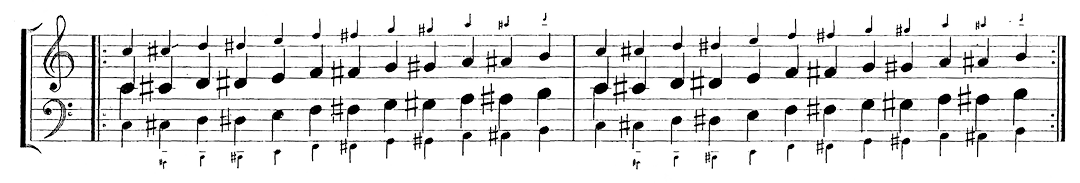
\includegraphics{img_148.png}
\caption[谢泼德音阶的两个完整周期的钢琴谱。]
  {谢泼德音阶的两个完整周期的钢琴谱。每个音符的音量与其大小成正比,因此,当最上面的声部消失时,下面一个新的声部出现了[该图为唐纳德·伯德的程序“斯马特”所印出] }
\end{sidewaysfigure}

这个奇妙的音乐发现使得“无穷升高的卡农”可以这样演奏:当它“升高”了一个八度之后,又回到了自身之中。这个主意是我和斯科特·凯姆一起想出来的,而且已经用一个计算机音乐系统实现在一盘磁带上了。其效果极其微妙——但非常寘实。有意思的是巴赫本人在某种意义下显然是知道这种音阶的,因为在他的曲子中不时能发现一些段落在大体上利用了谢泼德音调的普遍原理——例如在他为管风琴所写的《G小调幻想曲和赋格中幻想曲》的中部。

汉斯·西奥多·大卫在他的著作《约·塞·巴赫的〈音乐的奉献〉》中写到:

\begin{quote}
在整部《音乐的奉献》中,读者、听众和演奏者始终都在寻找各种形式的国王主题。因此这个作品可以说是一部名副其实、不折不扣的“探求曲”。\note{汉·西·大卫,《约·塞·巴赫的〈音乐的奉献〉》,第34页。}
\end{quote}

我认为这是真实的。没人能把《音乐的奉献》看透。当一个人自以为知道了其中的一切的时候,总还有他所不知道的东西。例如,在其中那个他不情愿即席演奏的六部无插入赋格的结尾处,他狡猾地把自己的名字藏在了上面两个声部之间。在《音乐的奉献》中,事情往往在许多层次上发展。有关于音符和字母的技巧,有国王主题的精巧变奏,有各种原始形式的卡农,有复杂得异乎寻常的赋格,有优美并极其深沉的情感,甚至还有由作品发展的多层次性所带来的喜悦。《音乐的奉献》是一部赋格的赋格,很像艾舍尔和哥德尔所构造的那种缠结的层次结构,是一个智慧的结晶。它以一种我无法表达的方式使我想起了人类思维这个美妙的多声部赋格。因此,我才在本书中把\emph{哥德尔}、\emph{艾舍尔}、\emph{巴赫}这三块我精心收\emph{集}的\emph{异}彩夺目的瑰\emph{璧}嵌为一体,并使\emph{之}发扬光大、辉映\emph{成}章。而这三块有\emph{异}曲同工之妙的奇珍,也因此凝\emph{集}成了一个珠联\emph{璧}合的整体。
